\documentclass{sigchi}

% \usepackage{amsmath}
% \usepackage{amsfonts}
% \usepackage{hyperref}
% \usepackage{graphicx}
% \usepackage{multirow}
% \usepackage{booktabs}

\usepackage{balance}  % to better equalize the last page
\usepackage{graphics} % for EPS, load graphicx instead
% \usepackage{times}    % comment if you want LaTeX's default font
\usepackage{url}      % llt: nicely formatted URLs
\usepackage{verbatimbox}

\makeatletter
\def\url@leostyle{%
  \@ifundefined{selectfont}{\def\UrlFont{\sf}}{\def\UrlFont{\small\bf\ttfamily}}}
\makeatother
\urlstyle{leo}

\def\pprw{8.5in}
\def\pprh{11in}
\special{papersize=\pprw,\pprh}
\setlength{\paperwidth}{\pprw}
\setlength{\paperheight}{\pprh}
\setlength{\pdfpagewidth}{\pprw}
\setlength{\pdfpageheight}{\pprh}

% Make sure hyperref comes last of your loaded packages,
% to give it a fighting chance of not being over-written,
% since its job is to redefine many LaTeX commands.
\usepackage[pdftex]{hyperref}
\hypersetup{
pdftitle={Kindsicher: Safe Internet Browsing for Unsupervised Children},
pdfauthor={LaTeX},
pdfkeywords={filter, children, snort, Internet},
bookmarksnumbered,
pdfstartview={FitH},
colorlinks,
citecolor=black,
filecolor=black,
linkcolor=black,
urlcolor=black,
breaklinks=true,
}

% create a shortcut to typeset table headings
\newcommand\tabhead[1]{\small\textbf{#1}}

% End of preamble. Here it comes the document.
\begin{document}

\title{Kindsicher: Safe Internet Browsing for Unsupervised Children}

\numberofauthors{3}
\author{
  \alignauthor Chaitanya Achan\\
    \affaddr{University of Utah}\\
    \email{cachan6460@gmail.com}\\
  \alignauthor Philip Lundrigan\\
    \affaddr{University of Utah}\\
    \email{philipbl@cs.utah.edu}\\
  \alignauthor Christian Schreiner\\
    \affaddr{University of Utah}\\
    \email{cas@cs.utah.edu}\\
}

\maketitle


% ############################################################################
% document body:

\begin{abstract}
% primary responsibility: CAS

In a modern society, children must increasingly use the Internet for required
tasks such as homework and communication with parents and other family
members, not just for optional tasks (such as games and entertainment). 
%
The amount of required use means that children must often use the Internet
when their parents cannot supervise them. 
%
This carries significant risk that the children will encounter Internet
content they are not able to handle, or that would exploit them. 
%
Most previous work on improving children's Internet safety focuses on
identifying ``bad'' content and blocking it. 
%
The amount of work to identify ``bad'' content is, however, beyond the
capabilities of most families. 
%
Commercial services exist that classify content, but they are still stretched
to adequately deal with the volume of legitimate content, and black hats are
continually finding new means of circumventing the services' products. 
%
Further, outsourcing content classification prevents a parent from restricting
content for family-specific reasons. 
%
For example, a child may have a phobia about spiders, or a parent may want to
insist on accompanying a child whenever they visit certain online shopping
sites, so the parent can teach good consumer practices during the shopping
session. 

We present Kindsicher, a children's Internet safety system that addresses
these issues by taking the opposite approach: parents define the Internet
sites they believe are appropriate for their children to visit unsupervised,
and access to other sites requires parental intervention. 
%
Kindsicher has the additional advantage that it is implemented as home network
infrastructure, so its protection is automatically extended to new devices
brought into the home (for example, when a friend arrives with a Wi-Fi
tablet). 


\end{abstract}

\keywords{
    Put keywords here
}

% primary responsibility: CAS


% force the word INTRODUCTION to not appear by itself at the end of a column
\vspace{20mm}

\section{Introduction}
\nopagebreak
In a modern society, children must increasingly use the Internet for required
tasks such as homework and communication with parents and other family
members, not just for optional tasks (such as games and entertainment).
%
The amount of required use means that children must often use the Internet
when their parents cannot continually supervise them.
%
This carries significant risk that the children will encounter Internet
content they are not able to handle, or that would exploit them.

Most previous work on improving children's Internet safety focuses on
identifying ``bad'' content and blocking it. Some of this work relies
on autoclassification (e.g. Dans Guardian~\cite{dansguardian}), some on
human classification (e.g. OpenDNS~\cite{opendns}), and some on a
combination (e.g. NetNanny~\cite{netnanny}).
%
The amount of work to identify ``bad'' content is, however, beyond the
capabilities of most families.

Commercial services exist that classify content~\cite{opendns, netnanny,
mcafee,k9}, but they are still stretched to adequately deal with the volume of
legitimate content, and black hats are continually finding new means of
circumventing the services' products.
%
It is disappointing to observe a pattern in commercial product literature of
focusing on features and testimonials, and omitting technical
details.~\cite{opendns, kidlogger, mcafee, k9}
%
This prevents parents (or a technically inclined friend of the parents) from
making a rational comparison between products and evaluating potential for
ineffectiveness or circumvention without purchasing each product and
performing detailed technical experiments.
%
Further, outsourcing content classification prevents a parent from restricting
content for family-specific reasons.
%
For example, a child may have a phobia about spiders, or a parent may want to
insist on accompanying a child whenever they visit certain online shopping
sites, so the parent can teach good consumer practices during the shopping
session.

This paper presents Kindsicher,\footnote{Kindsicher is a portmanteau of the
German words for ``child'' and ``safe.''} a children's Internet safety system
that addresses these issues by taking the opposite approach: 
%
parents define the Internet sites they believe are appropriate for their
children to visit unsupervised, and access to other sites requires parental
intervention.
%
Kindsicher offers the following advantages:

\begin{itemize}

\item Kindsicher allows the parents full control over the Internet sites to be
designated as ``safe''.
%
Kindsicher's architecture allows for parents to define exceptions to the
approved site list so children can browse additional content when parents
are present.
%
It would be conceptually simple to extend this so parents could temporarily
add sites via a web-capable smartphone, in case children needed to access
another site while their parents were away.

\item Kindsicher is completely implemented as part of a home network
infrastructure, so its protection is automatically extended to new
devices brought into the home (for example, when a friend arrives
with a Wi-Fi tablet). Most other solutions have a component that
must be installed on the client device.

\item Since Kindsicher is completely implemented on the home
network, it does not slow network performance while content is
routed via a cloud-based filtering server.  This can be a factor for
current and modern rich-content web pages.

\item Kindsicher logs all Internet traffic, so parents can have a rational
conversation with their children if a problem occurs.
%
(Problems might range from a teenager excessively playing online games, to a
child coming to parents in tears because something seen on the Internet
scared him/her.)

\item Kindsicher's logging feature means that if black hat malware tried to
attack the Kindsicher server, the attack would be logged, so technically
competent humans could address the problem.
%
Even a non-technically inclined parent could still see which computer in the
home was involved in the attack (either as a source or as a victim), and take
that computer to a repair shop for malware removal and an anti-virus update.

\item Kindsicher blocks traffic by interrupting TCP connections, as
opposed to blocking DNS name lookups, so it cannot be circumvented
by hard-coding an IP address in a URL (e.g. http://155.98.65.24/),
which is a common black-hat tactic.

\item Kindsicher is completely open-source software, so the
technically inclined are free to examine it, improve it if desired,
and share their results with others.

\end{itemize}

No product or system exists today that has all of these features. We hope that by developing Kindsicher, we can show that each of these features is important and should be integrated into previous systems.

% primary responsibility: CAS+Phil

\section{Related Work}

% primary responsibility: CAS+Phil

\section{Design}




\subsection{Login}

The TCP/IP protocol, and the HTTP protocol that rides on top of it, identify
the sending computer, \emph{NOT} the user name on that computer.  
% 
Since Kindsicher's goal is to restrict access for children, not for adults,
the only way to distinguish between children's internet access and adults'
access is to designate certain computers for children's use only, and other
computers for adults' use only.  
%
Thus, there needs to be some mechanism to ensure that the children can only
log into hosts designated for children.

The network we used for testing uses SNISR 
%
\footnote{ SNISR is a network login and directory information system, akin to
LDAP, NIS, or Hesiod.  Its signature advantage is that all clients have a
local record of account and group information at all times, so mobile clients
can be disconnected from the network and reconnected at will.  For more
information, see http://www.mathoni.net/cas/swforge/snisr for more
information. }
%
for login directory services.  
%
The current released version, SNISR 1.1, allows any user to log in on any host.  
%
Part of this project, therefore, was upgrading SNISR to allow the network
administrator to specify classes of hosts that only certain users could log
into.
%
SNISR 2.0's baseline ALPHA_6 contains this feature, and is expected to begin
beta testing soon.



% primary responsibility: Phil

\subsection{Blocking}

Figure~\ref{fig:rule_syntax} shows the general syntax for a Snort rules. There are eight types of snort rules: alert, log, pass, active, dynamic, drop, reject, and sdrop. Each type is described below:

\begin{itemize}
    \item \textbf{Alert}.
        Alert is the most commonly used type of rule. It sends an alert to the
        network to who ever is running the Snort server \emph{and} logs the
        packet(s) for later inspection.

    \item \textbf{Log}.
        Log logs the packet, but does not send an alert.  This can be used for
        a rule that is not critical but the network administrator wants to be
        able to look at it later.

    \item \textbf{Pass}.
        Pass does not do anything with the packet. The packet is ignored and
        allowed to proceed to its destination.

    \item \textbf{Active}.
        The is the same as Alert except that after sending an alert, a dynamic
        rule is turned on.

    \item \textbf{Dynamic}.
        A dynamic rule will do nothing until activated by an Active rule. Once
        it has been activated, it asks as a log rule

    \item \textbf{Drop}.
        Drop blocks the packet and logs it.

    \item \textbf{Reject}.
        Reject blocks the packet, logs it, and sends a TCP reset message (for a
        TCP connection) or a ICMP port unreachable message (for UDP connection)
        to both ends of the connect.

    \item \textbf{sDrop}.
        Same as Drop except that the packet is not logged.
\end{itemize}

For the purposes of blocking websites, we are interested in drop, reject, and
sdrop. We want to be record when a website is being blocked (we want the packet
logged), sdrop does not fit our needs. For drop to work correctly, Snort needs
to configured in inline mode. Inline mode is when the Snort server is inline
with Internet traffic. For example, the Snort server would be between the local
network and the Internet connection. Add data is inspected by the server and
either blocked or passed through. As our design section describes, this
configuration has important implications. This means that if the Snort server
fails then the Internet connection will be lost. This also means that the Snort
server could potentially act as a bottle neck, slow down traffic. Because of
these reasons, we decided that putting Snort inline in the network did not fit
our needs. This means that block is not a valid action.

The last rule action is reject. Since we are concerned about rejecting HTTP
requests, we concern ourselves with only the TCP functionality of reject and
ignore the UDP functionality. Reject uses a well studied TCP attack called TCP
Reset attack~\cite{watson2004slipping}.

\begin{figure}[!t]
    \centering
    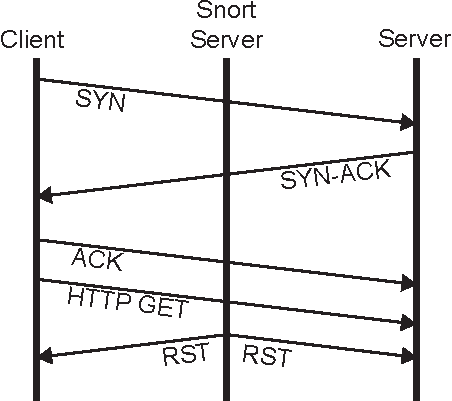
\includegraphics[width=.8\columnwidth]{figures/tcp_reset}
    \caption{The flow of how a TCP RST attack works in our system. When the
    Snort server detects a HTTP GET request, the Snort server sends a TCP RST
    packet to both ends of the connection (Client and Server).}
    \label{fig:tcp_reset}
\end{figure}

For a TCP Reset attack to work, there must be a man in the middle. It monitors
the TCP connections that are being made between the network and the Internet.
When the man in the middle wants to top a connection, it sends a TCP RST packet
to both ends of the connections. Both ends of the connection think that the
packet came from the other end so it honors the RST packet. For this to work,
the man in the middle must know the sequence number and ACK number of the TCP
stream. This can easily be found by looking at the header of TCP packets. Once
both ends of the connect receive the TCP RST packet, they stop sending data and
close the connection. Figure~\ref{fig:tcp_reset} shows a packet flow of a TCP
reset attack.

For the cause of Snort, the Snort server is the man in the middle. When a
reject rule is triggered, the Snort server sends a TCP RST packet to each end
of the connection.

\begin{figure}[!t]
    \centering
    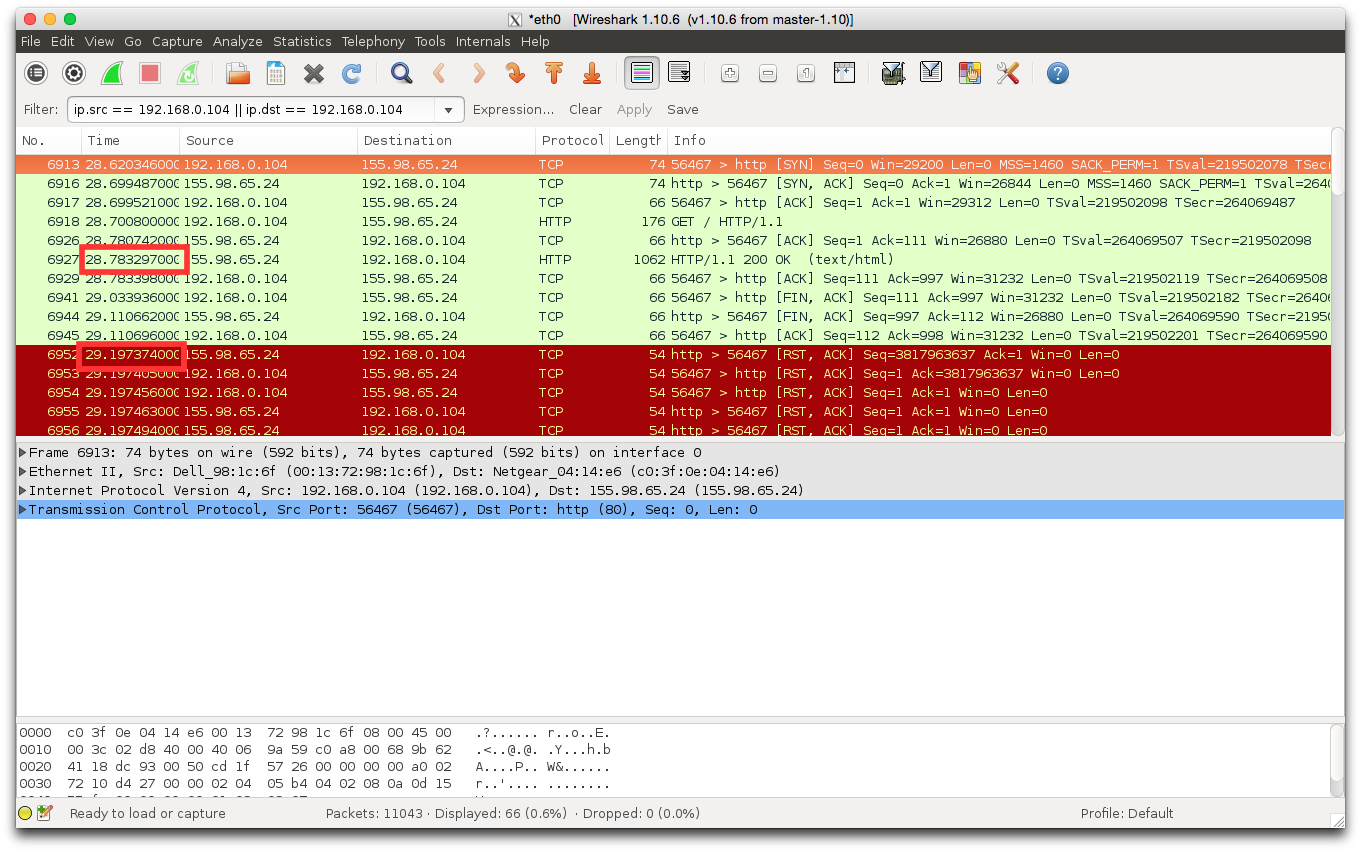
\includegraphics[width=\columnwidth]{figures/snort_slow}
    \caption{A screen shot of a Wireshark trace. In this trace, the Snort
    server is .41 seconds too late in sending TCP RST packets.}
    \label{fig:snort_slow}
\end{figure}

Snort's reject rule works in theory, but in practice it has some problems. An
inherent issue with not having our Snort server inline but instead having it
rejecting connections is that there could be conditions such that a TCP
connection could transmit data before the Snort server has time to respond.
This is exactly what happens under certain conditions.
Figure~\ref{fig:snort_slow} shows a screen shot of a Wireshark trace. In it,
the TCP connection is established, data is sent, and then the Snort server
sends its TCP RST packets. The time between when the data is received by the
client and when the Snort server sends a TCP RST packet is .41 seconds.

To really understand the problem with Snort being slow, we ran Snort in many
different environments to make sure it wasn't a platform or topology specific
problem. We ran the server on a MacBook Pro running OS X 10.10, a home network
server running Ubuntu 14.04, and on an Emulab~\cite{emulab} node running Ubuntu
14.04. In the first two environments, the same problems occurred -- Snort would
not react fast enough to block all TCP traffic. In the third environment, we
couldn't test a web server on the Internet (because of how Emulab is set up),
but Snort was able to block a web server that was part of the Emulab
experiment.

After some experimentation, there seems to be two factors that play a role in
if the Snort server is able to reject a TCP connection or not. The first is the
latency involved in making the request. If the request is being made to a
server that is near by geographically, the Snort server has a harder time
blocking it because the connection is so fast. The second factor is how big the
web page that is being downloaded. In our tests, we found that Snort was unable
to block web pages that could be contained inside one TCP packet. However, if
web page was large enough that there needed to be a few packets to send the
data, then Snort could block it most of the time. This was also true with large
images as well.

To try to minimize this problem, we tried reducing the functionality of Snort.
Snort is a IDS and has a lot more functionality that we don't need to block
websites. By reducing what Snort is loading in its configuration, we can speed
up the response time of the TCP RST packets. This helped to reduce the problem,
but it did not fix it. In the future, we plan on looking at the source code of
Snort and pulling out only the necessary parts to block websites.


\subsection{Whitelist}

\begin{figure}[!t]
    \centering
    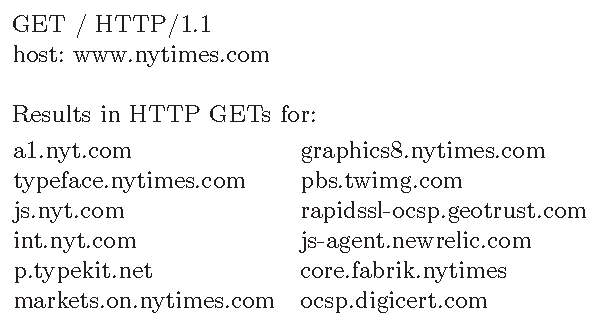
\includegraphics[width=\columnwidth]{figures/http_get}
    \caption{One HTTP GET request results in many more HTTP GET requests. Some
    of these requests are to different domains.}
    \label{fig:http_get}
\end{figure}

Part of being able to block websites adequately, is being able to produce a
good list of URLs that should not be blocked (a whitelist). This is harder than
it first sounds. This is in part due to the complexities of the Internet.
Typically, when a web page is visited, resources from many different locations
are loaded. An example of this is shown in Figure~\ref{fig:http_get}. This
makes creating a realistic whitelist much more difficult.

To understand what a whitelist might look like for a typical family, one of the
authors allowed for their families Internet traffic to be logged. This was done
by using \texttt{tshark}~\cite{tshark} (a terminal version of Wireshark) to
monitor Internet traffic and output the host name of a HTTP GET request to a
file. This gave us insight into what kind of considerations need to be made
when building an accurate whitelist.


\subsection{Reporting}

The second goal of this project is to provide parents with the ability to
monitor and derive reports on their child's Internet access. 
%
We looked at incorporating BASE (Basic Analysis and Security Engine) into Kindsicher to
render this functionality. 
%
BASE is based of the ACID (Analysis Console for Intrusion Databases) project
and provides a web-based front-end to query and analyze alerts generated by
the SNORT IDS system.

We first define a rule within SNORT to capture all HTTP traffic originating
from the home network.  

\verb+alert tcp any any <> any 80 (msg:"HTTP Alert")+ 

This causes SNORT to log all HTTP requests from any source IP and port to any
destination IP and port 80 (indicating HTTP) to a MySQL database. 
%
BASE then reads the alert information from this database and displays it in a
web-browser. (Figure R1)

\begin{figure}
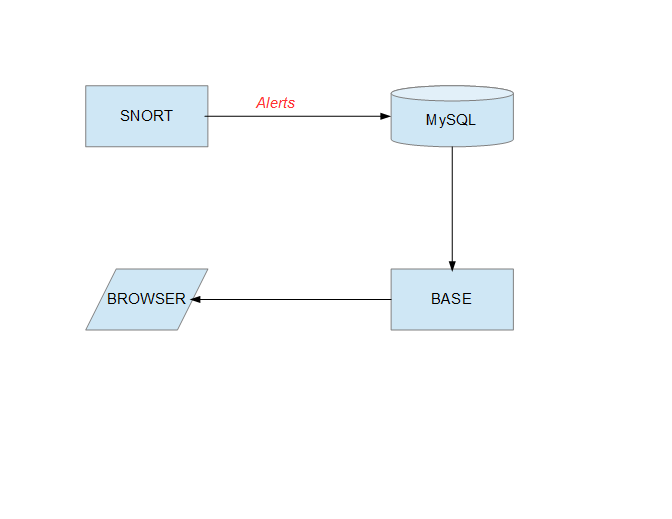
\includegraphics{figures/R1_BASE_Flow}
\end{figure}

% TODO: do something to label this R1 or similar

To access base you need to open a browser window and type in “<base server
name>/base” in the URL field.
%
Figure R2 shows the BASE home page presented to an user on logging into BASE.

% primary responsibility: Chaitu

\section{Future Work}

As described in the blocking section, we encountered some latency issues with
Snort that inhibited its blocking ability under certain conditions. For
Kindsicher to be effective in all circumstances, we need to investigate Snort
further. This might involve modifying the source of Snort to remove all extra
functionality. This could also involve writing our own program that blocks
using TCP Resets.

In the Reporting section, we described some of the shortcomings of BASE,
primary of which being its reporting on network access using only IP addresses.
The reporting can be made more user friendly by incorporating domain names
instead of or in addition to IP addresses. It could also be modified to provide
a richer set of data to parents, that makes understanding their child's web
access footprint much more intuitive.

Over the longer term, we also need a process that automates maintaining the
addresses in the Snort white-list. We envision that a child can request
addition of a new website domain as a text message to the parent's phone and
the parent could then chose to approve or deny that request, automatically
updating the white-list as needed. This would allow parents to change the
whitelist with minimal effort.

% primary responsibility: Phil

\section{Conclusion}

We present a system called Kindsicher that provides an unique approach to
protecting children from the potential harms of the Internet. Our system has
two major goals: block all access to websites, except for sites that are on a
white list and provide insight into how families are using the Internet through
reporting. We describe each of the components to our system and how they fit
together.

Over the course of designing the system, we found that building such a system
is much harder than first assumed. The Internet is a complex place which makes
it hard to build a system like this that is robust enough to withstand real
usage.

\proposedtext{At the same time, that very complexity makes it ever so much
more important for children to learn how to handle the advantages and risks
that the Internet offers.  A fully functional Kindsicher system would be a
useful tool to help parents teach their children how to deal with it.}
\{TODO: Phil: do you concur with this proposed text?\}

\{TODO: make this last paragraph appear on the same page with one of the figures.}


\balance

\bibliographystyle{acm-sigchi}
\bibliography{../project}

% ############################################################################
\end{document}

%%% Local Variables:
%%% mode: latex
%%% TeX-master: "root"
%%% End:
